%  cpu.tex
%  Document created by seblovett on octopus
%  Date created: Thu 03 Apr 2014 12:56:02 BST
%  <+Last Edited: Fri 04 Apr 2014 15:38:15 BST by hl13g10 on octopus +>

%\section{Processor}

%The whole processor is pulled together in two encapsulating modules. 
%The datapath module links the registers and ALU and implements the data multiplexors, program counter and accumulator.
%The top level CPU module links the program ROM, controller and datapath. 

\section{Datapath}\label{sect:datapath}
\subsection{Testbench}
%\todo[inline]{Explain testbench}
The testbench verifies the following: %conducts the following tests:
\begin{enumerate}
\item Program counter increment and write enable
\item Immidate loading into accumulator
\item Addition with an immediate
\item Write back to register
\item Read from register
\item Store switches to registers
\item Read switches from register
\item Program counter jump to accumulator value
\end{enumerate}

These operations are verified by viewing the LED output (the accumulator) and the program counter.
Assertions are used to check the outputs and keep an error count. 
This testbench is to check the internal connections of the datapath, and also the implementation of the extra registers.
Figure \ref{fig:datapathsim} shows the waveform of the simulation. 
The error count remains zero through out showing no errors exist in the datapath.
%\subsection{Simulation}
%\todo[inline]{Simulation Results}

\begin{figure}
\includegraphics[height=\textheight-1cm]{Figures/datapathsim.eps}
\caption{Datapath simulation waveform}
\label{fig:datapathsim}
\end{figure}

\subsection{Synthesis}
%\todo[inline]{Synthesis}

The synthesis of the datapath creates an instance of the register and ALU. 
It also implements the accumulator and program counter. 
A large number of multiplexors are used to direct the dataflow.% and all are 8 bit, 2:1 multiplexors. 
These take up a significant amount of the datapath. 
The whole synthesis is shown in figure \ref{fig:datapathsynth}.


\begin{figure}
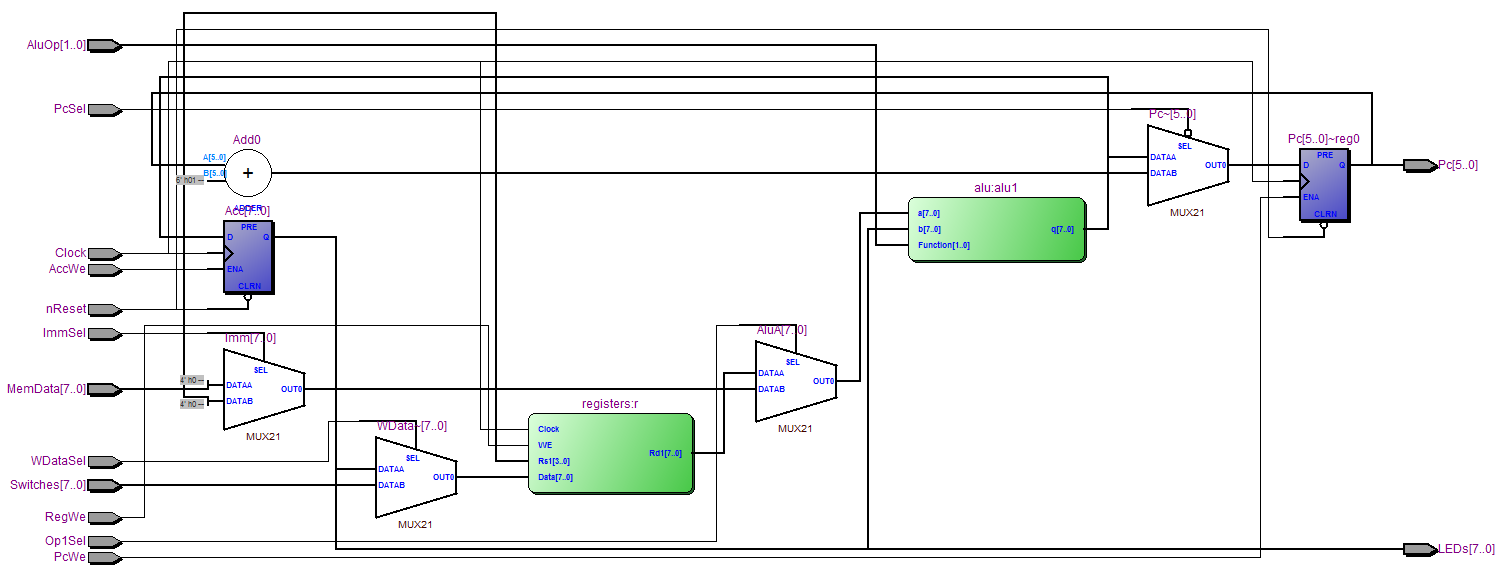
\includegraphics[width=\textwidth]{Figures/datapathsynth.png}
\caption{Synthesis of the Datapath}
\label{fig:datapathsynth}
\end{figure}


\section{CPU}
\subsection{Testbench}
%\todo[inline]{Describe testbench}

The testbench has two main parts; a task to commence the handshaking protocols, and a function to calculate the expected result. 
The handshaking task also contains assertions to verify the output. 
The function contains the constants and calculates the transform, with correct rounding.
The task can be seen in listing \ref{lstcputask} and the function is shown in listing \ref{lstcpufunction}.
These are used in a loop to test random sets of inputs. 
A few basic tests are also done with simple data. 

\lstinputlisting[firstline=31,style=sverilog,lastline=63,caption={Verification task to conduct the handshaking protocols. Assertions are used in this task to verify the output.},label=lstcputask]{../Implementation/cpu_stim.sv}
\lstinputlisting[style=sverilog,firstline=65, lastline=81,caption={Function used to calculate the expected output of the affine transform.},label=lstcpufunction]{../Implementation/cpu_stim.sv}




\subsection{Simulation Results}
%\todo[inline]{Full System Test}

Figure \ref{fig:cpusim} shows the output waveform of the test. 
Registers 0-5 contain the constants used. 
Registers 6 and 7 are used to store the initial $x_1$ and $y_1$ vector. 
Registers 9 and 10 are used to store the result and register 8 is used as a temporary register. 
The global error counter is shown, indicating that the whole system passes the test. 
Each iteration consists of a function call to calculate the expected outcome, and a task call to input the data. 
This process is then looped to test different datasets. 

\todo[inline]{Make a table of given inputs and expected outputs (real and rounded?)}

\begin{figure}
\includegraphics[height=\textheight-1cm]{Figures/cpusim.eps}
\caption{CPU simulation waveform}
\label{fig:cpusim}
\end{figure}

\subsection{Synthesis}
%\todo[inline]{Full system synthesis}

The top level module creates a instance of the controller, datapath and ROM. 
The interconnects are made here and the inputs and outputs to the controller are also made.
This top level synthesis is shown in figure~\ref{fig:cpusynth}.


\begin{figure}
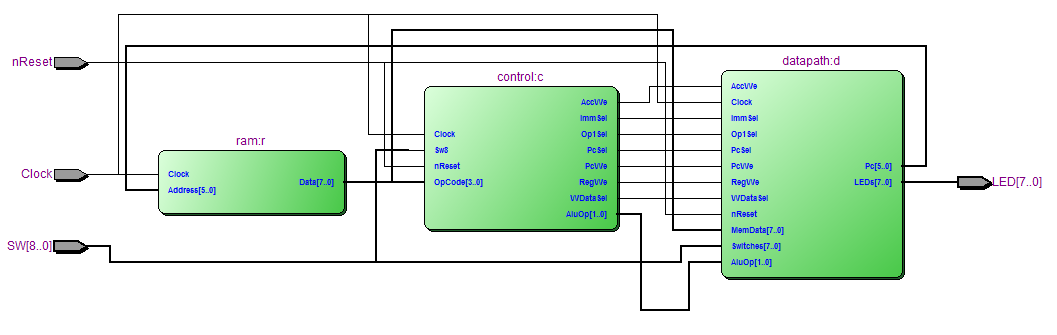
\includegraphics[width=\textwidth]{Figures/cpusynth.png}
\caption{Top level synthesis of the processor.}
\label{fig:cpusynth}
\end{figure}

